\subsection{Mixed Integer Non Linear Programming Formulations}\label{Form}
% \JP{In this section we present a MINLP formulation for the (\AMD). Let us denote by $\mathcal T$ the set of stages/tasks that the mothership and the fleet of drones have to carry out. These stages are visits to the different graphs in $\mathcal G$ with the required constraints. A stage $t\in\mathcal T$ is referred to as the operation in which the mothership launches some drones from a taking-off location, denoted by $x_L^t$ and later it takes them back on a rendezvous location $x_R^t$. Here, it is important to realize that both locations $x^L_t$ and $x^R_t$ must be determined in the continuous space where the mothership is assumed to move. Note that $|\mathcal T|\leq|\mathcal G|$, since it is assumed that, for each stage, at least one drone must be launched. Clearly, the distance $d_{LR}^t$ traveled by the base vehicle for the stage $t$, i.e., to go from $x_L^t$ to $x_R^t$ is
% $$d_{LR}^t=\|x_L^t - x_R^t\|,$$
% where $\|\cdot\|_2$ denoted the Euclidean distance,  although this assumption can be extended to any $l_p$ norm, $1\leq p\leq \infty$.} 
\noindent
In this section we present a MINLP mathematical programming formulation for the \AMD %\;\hspace{-2}%  
that can be used to solve medium size instances of this problem.
\noindent
As mentioned in Section \ref{section:desc}, we assume that the mothership is allowed to move freely in a continuous space that for the sake of presentation we  assume to be $\mathbb R^2$. Here, distances are measured by the Euclidean norm, $\|\cdot\|_2$, although this assumption can be extended to any $l_p$ norm, $1\leq p\leq \infty$ (see \cite{Blanco2017}).
\noindent
In the following, we introduce the parameters or input data that formally describe the problem and that are summarized in Table \ref{table:t1}.

 \begin{table}[!h]
\scriptsize
\centering
%\color{blue}
\begin{tabular}{ | l | }
\hline
\textbf{Problem Parameters}\\
\hline
$origin$: coordinates of the point defining the origin of the mothership path (or tour).\\
$dest$: coordinates of the point defining the destination of the mothership path (or tour).\\
$\mathcal{G}$: set of the target graphs.\\
$g = (V_g, E_g)$: set of nodes and edges of each target graph $g \in \mathcal{G}$.\\
$\mathcal{L}(e_g)$: length of edge $e$ of graph $g \in \mathcal{G}$.\\
$\mathcal{L}(g)=\sum_{e_g\in E_g} \mathcal L(e_g)$: total length of the graph $g\in\mathcal G$.\\
$B^{e_g}, C^{e_g}$: coordinates of the endpoints of edge $e$ of graph $g \in \mathcal{G}$.\\
$\alpha^{e_g}$: percentage of edge $e$ of graph $g \in \mathcal{G}$ that must be visited.\\
$\alpha^{g}$: percentage of graph $g \in \mathcal{G}$ that must be visited.\\
$v_D$: drone speed.\\
$v_M$: mothership speed.\\
$N^d$: drone endurance. \\
$M$: big-M constant.\\
\hline
\end{tabular}
\caption{Nomenclature for AMMDRPG}
\label{table:t1}
\end{table}

\begin{table}[h!]
%\tiny
\scriptsize
\centering
%\color{blue}
\begin{tabular}{|l|}
\hline 
\textbf{Binary and Integer Decision Variables}\\
\hline
$\mu^{e_g} \in \{0,1\} \:\: \forall e_g \in E_g$ ($g \in \mathcal{G}$): equal to 1 if edge $e$ of graph $g$ (or a portion of it) is visited by the drone,\\ \hspace*{1cm} and  0 otherwise.\\
$\text{entry}^{e_g} \in \{0,1\} \:\: \forall e_g \in E_g$ ($g \in \mathcal{G}$): auxiliary binary variable used for linearizing expressions.\\
$u^{e_{g}td} \in \{0,1\} \:\: \forall e_g \in E_g$ ($g \in \mathcal{G}$) $\: \forall t \in \mathcal T \: \forall d \in \mathcal D$: equal to 1 if the drone $d$ enters in graph $g$ by the edge $e_g$ at stage $t$,\\ \hspace*{1cm} 0 otherwise.\\
$z^{e_{g}e^{'}_{g}} \in \{0,1\} \:\: \forall e_g, e_g' \in E_g$ ($g \in \mathcal{G}$): equal to 1 if the drone goes from $e_g$ to $e^{'}_{g}$, 0 otherwise.\\
$v^{e_{g}td} \in \{0,1\} \:\: \forall e_g \in E_g$ ($g \in \mathcal{G}$) $\: \forall t \in\mathcal T \: \forall d \in \mathcal D$: equal to 1 if the drone $d$ exits from graph $g$ by $e_g$ at stage $t$,\\ \hspace*{1cm} 0 otherwise.\\
$s^{e_g},\; \forall e_g \in E_g$ ($g \in \mathcal{G}$): integer non negative variable representing the order of visit of the edge $e$ of graph $g$.\\
\hline
\textbf{Continuous Decision Variables}\\
\hline
$\rho^{e_g} \in [0,1]$ and $\lambda^{e_g} \in [0,1] \:\: \forall e_g \in E_g$ ($g \in \mathcal{G}$): defining the entry and exit points on $e_g$.\\
$\nu_\text{min}^{e_g}$ and $\nu_\text{max}^{e_g} \in [0,1] \forall e_g \in E_g$ ($g \in \mathcal{G}$): auxiliary variables used for linearizing expressions.\\
$x_L^t \:\: \forall t \in\mathcal T$: coordinates representing the point where the mothership launches the drone at stage $t$.\\
$x_R^t \:\: \forall t \in\mathcal T$: coordinates representing the point where the mothership retrieves the drone at stage $t$.\\
$R^{e_g} \:\: \forall e_g \in E_g$ ($g \in \mathcal{G}$): coordinates representing the entry point on edge $e$ of graph $g$.\\
$L^{e_g} \:\: \forall e_g \in E_g$ ($g \in \mathcal{G})$: coordinates representing the exit point on edge $e$ of graph $g$.\\
$d_L^{e_gtd} \geq 0, \:\: \forall e_g \in E_g$ ($g \in \mathcal{G}$) $\forall t \in\mathcal T \:\forall d\in\mathcal D$: representing the distance travelled by the drone $d$ from the launching\\
\hspace*{1cm} point $x_L^t$ on the mothership at stage $t$ to the first visiting point $R^{e_g}$ on $e_g$.\\
$d^{e_ge^\prime_g} \geq 0, \:\: \forall e_g, e^\prime_g \in E_g $ ($g \in \mathcal{G}$): representing the distance travelled by the drone from the launching\\
\hspace*{1cm} point $L^{e_g}$ on $e_g$ to the rendezvous point $R^{e^\prime_g}$ on $e^\prime_g$.\\
$d^{e_g} \geq 0, \:\: \forall e_g \in E_g$ ($g \in \mathcal{G}$): representing the distance travelled by the drone from the rendezvous\\
\hspace*{1cm} point $R^{e_g}$ to the launching point $L^{e_g}$ on $e_g$. \\
$d_R^{e_gtd} \geq 0 \:\: \forall e_g \in E_g$ ($g \in \mathcal{G}$) $\forall t \in\mathcal T\:\forall d\in\mathcal D$: representing the distance travelled by the drone $d$ from the last\\
\hspace*{1cm} visiting point $L^{e_g}$ on $e_g$ to the rendezvous point $x_R^t$ on the mothership at stage $t$.\\
$d_{LR}^t \geq 0 \:\: \forall t \in\mathcal T$: representing the distance travelled by the mothership from the \\
\hspace*{1cm} launching point $x_L^t$ to the rendezvous point $x_R^t$ at stage $t$.\\
$d_{RL}^t \geq 0 \:\: \forall t \in\mathcal T$: representing the distance travelled by the mothership from the \\ 
\hspace*{1cm} rendezvous point $x_R^t$ at stage $t$ to the launching point $x_L^{(t+1)}$ at the stage $t+1$.\\
\hline
\end{tabular}
\caption{Decision Variables for AMMDRPG}
\label{table:t2}
\end{table}

\noindent
To represent the movement of the drone within a graph $g\in\mathcal G$, we proceed to introduce some notation related to $g$.
Let $g = (V_g, E_g)$ be a graph in $\mathcal G$ whose total length is denoted by $\mathcal L(g)$. Here, $V_g$ denotes the set of nodes and $E_g$ denotes the set of edges connecting pairs of nodes. Let $e_g$ be the edge $e$ of the graph $g \in G$ and let $\mathcal  L(e_g)$ be its length. Each edge $e_g$ is parameterized by its endpoints $B^{e_g}= (B^{e_g}(x_1), B^{e_g}(x_2))$ and $C^{e_g}= (C^{e_g}(x_1), C^{e_g}(x_2))$ and we can compute its length $\mathcal L(e_g) =\|C^{e_g} -  B^{e_g}\|$.

% We shall refer to $e_g$  as a generic edge $e$ of this graph $g$. The  edge $e_g$ is determined by its endpoints $B^{e_g}, C^{e_g}$ and its length $\|\overline{B^{e_g}C^{e_g}}\|$ is denoted by $\mathcal L(e_g)$. For each edge $e_g$, we assign a binary variable $\mu^{e_g}$ that indicates whether or not the drone visits $e_g$. In addition, for each edge $e_g$ we define an entry $(R^{e_g}, \rho^{e_g})$ and an exit point $(L^{e_g}, \lambda^{e_g})$, being $\rho^{e_g}$ and $\lambda^{e_g}$ the values in the parametrization of the edge $e_g$ where the drone enters and leaves the edge. \\
\noindent
As discussed in Section \ref{section:desc}, we consider two modes of visit to the target graphs $g\in \mathcal{G}$:
\begin{itemize}
    \item Visiting a percentage $\alpha^{e_g}$ of each edge $e_g$ which can be modeled by using the following constraints:
    \begin{equation}\label{eq:alphaE}\tag{$\alpha$-E}
    |\lambda^{e_g} - \rho^{e_g}|\mu^{e_g}\geq \alpha^{e_g}, \quad \forall e_g\in E_g.
    \end{equation}
    \item Visiting a percentage $\alpha^g$ of the total length of the graph:
    \begin{equation}\label{eq:alphaG}\tag{$\alpha$-G}
    \sum_{e_g\in E_g} \mu^{e_g}|\lambda^{e_g} - \rho^{e_g}|\mathcal L(e_g) \geq \alpha^g\mathcal L(g).
    \end{equation}
   % \CV{where $\mathcal L(g)$ denotes the total length of the graph., this is mentioned before}
\end{itemize}

\bigskip
\noindent
In both cases the corresponding constraints are nonlinear. In order to linearize them, we need to introduce a binary variable $\text{entry}^{e_g}$ that determines the traveling direction on the edge $e_g$ as well as the definition of the parameter values $\nu_\text{min}^{e_g}$ and $\nu_\text{max}^{e_g}$ of the access and exit points to that segment. Then, for each edge $e_g$, the absolute value constraint \eqref{eq:alphaE} can be represented by:

\begin{equation}\label{eq:alpha-E}\tag{$\alpha$-E}
 \mu^{e_g}|\rho^{e_g}-\lambda^{e_g}|\geq \alpha^{e_g} \Longleftrightarrow
 \left\{
 \begin{array}{ccl}
  \rho^{e_g} - \lambda^{e_g}                       & =    & \nu_\text{max}^{e_g} - \nu_\text{min}^{e_g},                                     \\
  \nu_\text{max}^{e_g}                         & \leq & 1-{\text{entry}^{e_g}},                                   \\
  \nu_\text{min}^{e_g}                      & \leq & {  \text{entry}^{e_g}},                                        \\
  \mu^{e_g}(\nu_\text{max}^{e_g} + \nu_\text{min}^{e_g} ) & \geq & \alpha^{e_g}.
  \\
 \end{array}
 \right.
\end{equation}

\noindent
The linearization of \eqref{eq:alphaG} is similar to \eqref{eq:alphaE} by changing the last inequality in \eqref{eq:alpha-E} by

\begin{equation}\label{eq:alpha-G}\tag{$\alpha$-G}
\sum_{e_g\in E_g} \mu^{e_g}(\nu_\text{max}^{e_g} + \nu_\text{min}^{e_g})\mathcal L(e_g)\geq \alpha^g\mathcal L(g).
\end{equation}

\noindent
To model this problem, we use stages identified with the order in which the different elements in the problem are visited. Let us denote by $\mathcal T$ the set of stages/tasks that the mothership and the fleet of drones have to carry out. These stages are visits to the different graphs in $\mathcal G$ with the required constraints. A stage $t\in\mathcal T$ is referred to as the operation in which the mothership launches some drones from a taking-off location, denoted by $x_L^t$ and later it takes them back on a rendezvous location $x_R^t$. Here, it is important to realize that both locations $x_L^t$ and $x_R^t$ must be determined in the continuous space where the mothership is assumed to move. Note that $|\mathcal T|\leq|\mathcal G|$, since it is assumed that, for each stage, at least one drone must be launched.
\noindent
For each stage $t\in\mathcal T$, each one of the drones launched from the mothership must follow a path starting from and returning to the mothership, while visiting the required edges of $g$. According to the notation introduced above, we write this generic path in the following form:

$$
x_L^t\rightarrow R^{e_g}\rightarrow L^{e_g}\rightarrow\ldots\rightarrow R^{e^\prime_g}\rightarrow L^{e^\prime_g}\rightarrow \ldots \rightarrow R^{e''_g} \rightarrow x_R^t\rightarrow x_L^{t+1}.
$$


\begin{figure}[h!]
\centering
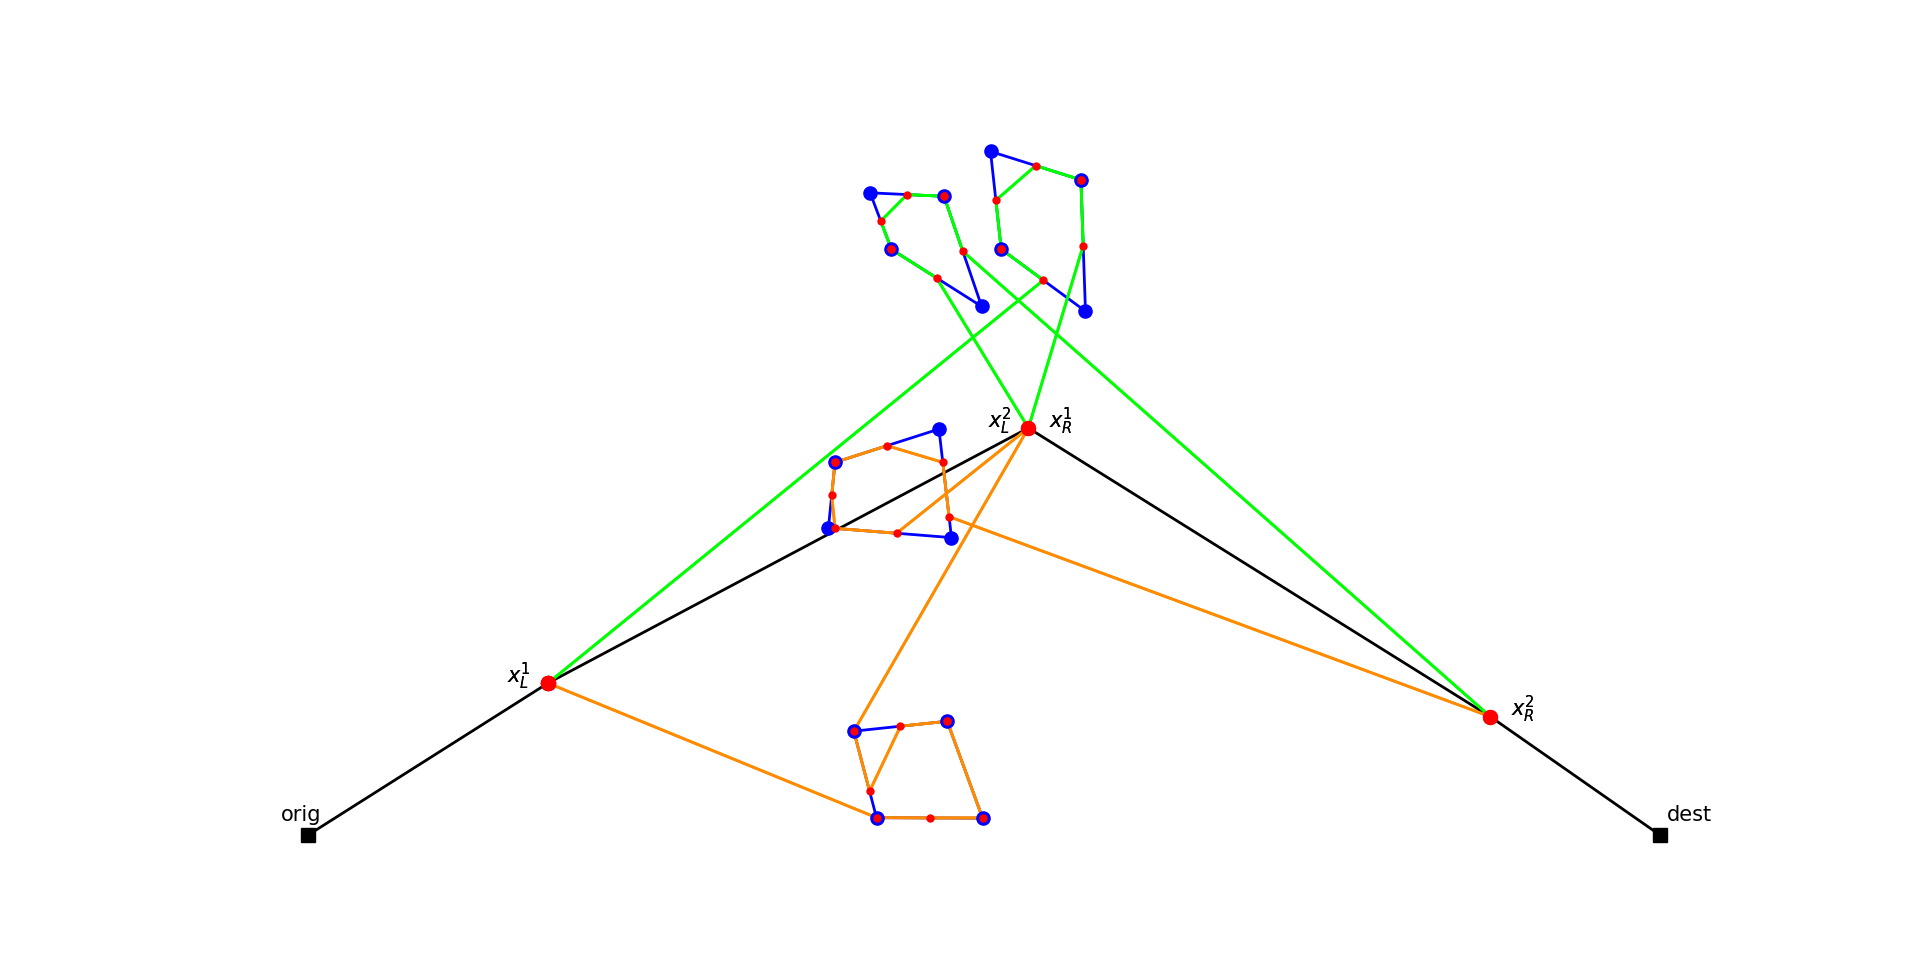
\includegraphics[width=0.95\linewidth]{figures/figure_latex.png}
\caption{Example illustrating the meaning of the launching  (L) and retrieving (R) points.}
\label{fig:illustrative}
\end{figure}

\noindent
Figure \ref{fig:illustrative} shows an example of the notation over a configuration with four target graphs that have four nodes and four edges. Here, it is supposed that the number of available drones is two. %: one with six nodes and 7 edges and the other one with four nodes and edges%. 
The mothership begins at its starting point $origin$. Then, it moves to $x_L^1$ where two drones are launched to visit two graphs. There, each drone follows a route (represented by the orange and green paths) that ensures the coverage of $50 \%$ of each edge of the graph. The red dots on the visited graphs are the intermediate points $R^{e_g}$ and $L^{e_g}$ used by the drones in their visit to the edges of the different graphs. After finishing the visit of the first two graphs the drones return to the point $x_R^1$ from where they are launched again to visit the remaining two graphs. Once these graphs are visited, the drones return to the mothership at the rendezvous point $x_R^2$ and then the mothership ends its route at the destination point $dest$.


% \JP{ ************************ 

% TO BE INSERTED: An example showing the notation with a figure...  Please Carlos insert something similar to what we use in the previous paper (JUSTO dixit)

%      ************************}
\noindent
To include the definition of these paths in our mathematical programming formulation we need to make decisions to choose:
\begin{itemize}
    \item The optimal assignment of drones for visiting graphs in a given stage $t$.
    \item The optimal order to visit the edges of each graph in its corresponding stage.
\end{itemize}

% Binary variables
% Thus, to this end one can define the following binary variables:
\noindent
We model the route that the drone follows by using the binary variables $u^{e_gtd}$, $z^{e_ge^\prime_g}$ and $v^{e_gtd}$ defined in Table \ref{table:t2}.


% \begin{itemize}
%   \item $u^{{e_g}td} = 1$ if the visit of graph $g$ is done at stage $t$ by the drone $d$ and it starts from edge $e_g$.
%   \item $v^{{e_g}td}= 1$ if the visit of graph $g$ that is done by drone $d$ at stage $t$ finishes in the edge $e_g$.
%   \item $z^{e_ge'_g}= 1$ if the drone moves from edge $e_g$ to $e'_g$ while visiting the graph $g$.
% \end{itemize}

% By using these binary variables, we can model the route that follows the drone:
\begin{align}
    \sum_{g\in \mathcal G}\sum_{e_g\in E_g} \sum_{d\in\mathcal D} u^{e_gtd} & \leq 1, &\forall t\in \mathcal T, \label{st:DEnt}\\%\tag{DEn}\\
    \sum_{g\in\mathcal G}\sum_{e_g\in E_g} \sum_{d\in\mathcal D} v^{e_gtd} & \leq 1, &\forall t\in \mathcal T, \label{st:DExt}\\%\tag{DEx}\\
    \sum_{e_g\in E_g} \sum_{t\in \mathcal T} \sum_{d\in\mathcal D} u^{e_gtd} & = 1, &\forall g\in\mathcal G, \label{st:DEng}\\%\tag{D
    \sum_{e_g\in E_g} \sum_{t\in \mathcal T} \sum_{d\in\mathcal D} v^{e_gtd} & = 1, &\forall g\in\mathcal G, \label{st:DExg}\\%\tag{D
    \sum_{e_g\in E_g} u^{e_gtd} & = \sum_{e_g\in E_g} v^{e_gtd}, &\forall g\in\mathcal G, \forall t\in \mathcal T, \forall d\in\mathcal D, \label{st:Duv}\\%\tag{D
     \sum_{t\in \mathcal T} \sum_{d \in \mathcal D} u^{e_gtd} + \sum_{e^\prime_g\in E_g} z_g^{e^\prime_ge_g} & = \mu^{e_g}, &\forall e_g\in E_g:g\in\mathcal G, \label{st:DInu}\\
     \sum_{t\in \mathcal T} \sum_{d \in \mathcal D} v^{e_gtd} + \sum_{e^\prime_g\in E_g} z_g^{e_ge^\prime_g} & = \mu^{e_g}, &\forall e_g\in E_g:g\in\mathcal G. \label{st:DInv}
\end{align}

\noindent 
Inequalities \eqref{st:DEnt} and \eqref{st:DExt} state that for each stage at most one drone can be launched and retrieved for performing an operation.  Constraints \eqref{st:DEng} and \eqref{st:DExg} assure that each graph is visited at some stage $t$ by some drone $d$. Equations \eqref{st:Duv} ensure that the operation of entering and exiting from the graph $g$ occurs in the same stage $t$ and is done by the same drone $d$. Constraints \eqref{st:DInu} state that 
if edge $e$ of graph $g$ is visited by the drone $d$, one of two alternative situations must occur: either $e$ is the first edge of graph $g$ visited by the drone $d$ at stage $t$, or edge $e$ is visited by the drone $d$ after visiting another edge $e^\prime$ of graph $g$. Similarly, constraints \eqref{st:DInv} state that if edge $e$ of graph $g$ is visited by the drone $d$, either $e$ is the last edge of graph $g$ visited by the drone at stage $t$, or the drone $d$ must move to another edge $e^\prime$ of graph $g$ after visiting edge $e$.
% Constraints \eqref{st:DInu} (resp. \eqref{st:DInv}) state that if the edge $e_g$ is visited, $\mu^{e_g}=1$, then either the drone enters coming from (leaves to) the mothership, $\sum_{t\in \mathcal T} \sum_{d \in \mathcal D} u^{e_gtd}=1$ ($\sum_{t\in \mathcal T} \sum_{d \in \mathcal D} v^{e_gtd}=1$), or it enters from (leaves to) another edge $e^\prime_g$, $\sum_{e^\prime_g\in E_g} z_g^{e^\prime_ge_g}=1$ ($\sum_{e^\prime_g\in E_g} z_g^{e_ge^\prime_g} =1$).

% A first attempt to model this problem uses stages identified with the order in which the different elements in the problem are visited. We identify each visit to one of the target graphs with a stage of the process. Then, by using the notation below, we define the stages set associated to graphs $T:=\{1,\ldots,|\mathcal G|\}$ and those associated to the launching and rendezvous points including $origin$ and $dest$ $T'=\{0,\ldots,|\mathcal G|+1\}$. For each stage $t\in T$, the drone follows the following path starting from the mothership, visiting the required edges of $g$ and returning to the mothership:

% $$
% x_L^t\rightarrow R^{e_g}\rightarrow L^{e_g}\rightarrow\ldots\rightarrow R^{e^\prime_g}\rightarrow L^{e^\prime_g}\rightarrow \ldots \rightarrow R^{e''_g} \rightarrow x_R^t\rightarrow x_L^{t+1}.
% $$

% This path calls in a natural way for the definition of binary variables that choose:
% \begin{itemize}
%     \item The optimal order to visit each graph $g\in\mathcal G$. In other words, defining the sequence of the stages.
%     \item The optimal order to visit the edges of each graph in its corresponding stage.
% \end{itemize}

% Thus, to this end one can define the following binary variables:
% \begin{itemize}
%     \item $u^{e_gt} = 1$ if the drone enters by the segment $e_g$ at the stage $t$.
%     \item $z^{e_ge^\prime_g} = 1$ if the drone goes from the segment $e_g$ to the segment $e^\prime_g$.
%     \item $v^{e_gt} = 1$ if the drone exits the graph by the segment $e_g$ at the stage $t$.
% \end{itemize}

% By using these binary variables, we can model the route that follows the drone:
% \begin{align}
%     \sum_{g\in \mathcal G}\sum_{e_g\in E_g} u^{e_gt} & = 1, &\forall t\in T \label{st:DEnt}\\%\tag{DEn}\\
%     \sum_{g\in\mathcal G}\sum_{e_g\in E_g} v^{e_gt} & = 1, &\forall t\in T \label{st:DExt}\\%\tag{DEx}\\
%     \sum_{e_g\in E_g} \sum_{t\in T} u^{e_gt} & = 1, &\forall g\in\mathcal G \label{st:DEng}\\%\tag{D
%     \sum_{e_g\in E_g}\sum_{t\in T} v^{e_gt} & = 1, &\forall g\in\mathcal G \label{st:DExg}\\%\tag{D
%     \sum_{e_g\in E_g} u^{e_gt} & = \sum_{e_g\in E_g} v^{e_gt}, &\forall g\in\mathcal G, \forall t\in T \label{st:Duv}\\%\tag{D
%     \sum_{e^\prime_g\in E_g} z_g^{e^\prime_ge_g} + \sum_{t\in T} u^{e_gt} & = \mu^{e_g}, &\forall e_g\in E_g:g\in\mathcal G \label{st:DInu}\\
%     \sum_{e^\prime_g\in E_g} z_g^{e_ge^\prime_g} + \sum_{t\in T} v^{e_gt} & = \mu^{e_g}, &\forall e_g\in E_g:g\in\mathcal G \label{st:DInv}
% \end{align}

% \noindent
% Equations \eqref{st:DEnt} and \eqref{st:DExt} state that in each stage the drone visits (enter and exit, respectively) only one graph. Constraints \eqref{st:DEng} and \eqref{st:DExg} assure that each graph is visited at some stage. Constraints \eqref{st:DInu} (resp. \eqref{st:DInv}) state that the number of exterior edges plus the number of interior edges that enter (resp. exit) to the edge $e_g$ is given by $\mu^{e_g}$.

\subsubsection*{Elimination of subtours}
\noindent
In order to represent actual routes of the drones over the target graphs, subtours cannot be allowed. Note that subtours would represent fake operations since they would allow free jumps of the drone between different routes at no time. To prevent the existence of subtours within each graph $g\in \mathcal G$ that the drone must visit, one can include, among others, either the compact formulation that uses the Miller-Tucker-Zemlin constraints (MTZ) or the subtour elimination  constraints (SEC).\\
\noindent
For the MTZ formulation, we use the continuous variables $s^{e_g}$, defined in Table \ref{table:t2}, that state the order to visit the edge $e_g$ and set the following constraints for each $g\in\mathcal G$:

\begin{align}
    s^{e_g} - s^{e^\prime_g} + |E_g|z^{e_ge^\prime_g} & \leq |E_g| - 1  , &\quad\forall e_g \neq e_g'\in E_g, \tag{MTZ$_1$} \label{MTZ1}\\
    0 & \leq s^{e_g} \leq |E_g| - 1, &\quad\forall e_g\in E_g.\tag{MTZ$_2$}\label{MTZ2}
\end{align}

\noindent
Alternatively, we can also use the family of subtour elimination constraints for each $g\in\mathcal G$:
\begin{equation}\tag{SEC}\label{SEC}
    \sum_{e_g, e^\prime_g \in S} z_g^{e_ge^\prime_g} \leq |S| - 1, \quad \forall S\subset E_g.
\end{equation}

\noindent
%(Copiado del XPPN)
Since there is an exponential number of SEC constraints, when we implement this formulation we need to perform a row generation procedure including constraints whenever they are required by a separation oracle. To find SEC inequalities, as usual, we search for disconnected components in the current solution. Among them, we choose the shortest subtour found in the solution to be added as a lazy constraint to the model.\\

\noindent
 The goal of the \AMD\xspace is to find a feasible solution that minimizes the total distance traveled by the mothership. To account for the different distances among the decision variables of the model we need to set the continuous variables $d_L^{e_gtd}$, $d^{e_g}$, $d^{e_ge^\prime_g}$, $d_R^{e_gtd}$, $d_{RL}^t$ and $d_{LR}^t$, defined in Table \ref{table:t2}. This can be done by means of the following constraints:
 
 %define the following instrumental variables:
% \begin{itemize}
%     \item $d_L^{e_gtd} = \|x_L^t - R^{e_g}\|$. Distance traveled by the drone $d$ from the launching point at the stage $t$ to the first visiting point in the segment $e_g$.
%     \item $d^{e_ge^\prime_g} = \|R^{e_g} - L^{e^\prime_g}\|$. Distance traveled by the drone $d$ from the launching point in $e_g$ to the next rendezvous point in the following edge $e^\prime_g$ of the graph $g$.
%     \item $d^{e_g} = \|R^{e_g} - L^{e_g}\|$. Distance traveled by the drone from the retrieving point  to the next launching point in $e_g$.
%     \item $d_R^{e_gtd} = \|L^{e_g} - x_R^t\|$. Distance traveled by the drone $d$ from the launching point in the last segment $e_g$ visited of the graph $g$ to the retrieving point on the mothership at the stage $t$.
%     \item $d_{LR}^t = \|x_L^t - x_R^t\|$. Distance traveled by the mothership from the launching point to the retrieving point at the stage $t$.
%     \item $d_{RL}^t = \|x_R^t - x_L^{t+1}\|$. Distance traveled by the mothership from the retrieving point at stage $t$ to the launching point at stage $t+1$.
% \end{itemize}

\begin{align*}
\|x_L^t- R^{e_g}\| & \leq  d_L^{e_gtd},  &\quad \forall e_g:g\in \mathcal{G}, \forall t\in \mathcal T, \forall d\in\mathcal D, \tag{DIST$_{1}$-t} \label{eq:d1}\\
\|R^{e_g}- L^{e_g}\| & \leq  d^{e_g},  &\quad \forall e_g:g\in \mathcal{G}, \tag{DIST$_{2}$-t} \label{eq:d2}\\
\|R^{e_g}- L^{e^\prime_g}\| & \leq  d^{e_ge^\prime_g}, &\quad \forall e_g\neq e_g'\in E_g:g\in \mathcal{G}, \tag{DIST$_{3}$-t} \label{eq:d3}\\
\|L^{e_g}- x_R^t\| & \leq  d_R^{e_gtd}, &\quad \forall e_g:g\in \mathcal{G},\forall t\in T, \forall d\in\mathcal D, \tag{DIST$_{4}$-t} \label{eq:d4}\\
\|x_R^t- x_L^{t+1}\| & \leq  d_{RL}^t, & \quad \forall t\in \mathcal T, \tag{DIST$_{5}$-t} \label{eq:d5}\\
\|x_L^t- x_R^t\| & \leq  d_{LR}^t, & \quad \forall t\in \mathcal T. \tag{DIST$_{6}$-t} \label{eq:d6}\\
\end{align*}

\noindent
The coordination between the drones and the mothership must ensure that the time spent by the drone $d$ to visit the graph $g$ at the stage $t$ is less than or equal to the time that the mothership needs to move from the launching point to the retrieving point during the stage $t$. To this end, we need to define the following coordination constraint for each graph $g\in \mathcal G$, stage $t\in \mathcal T$ and drone $d\in\mathcal D$:

\begin{equation}\tag{DCW}\label{DCW}
\frac{1}{v_D}\left(\sum_{e_g\in E_g} u^{e_gtd}d_L^{e_gtd} + \sum_{e_g, e^\prime_g\in E_g}z^{e_ge^\prime_g}d^{e_ge^\prime_g} + \sum_{e_g\in E_g} \mu^{e_g}d^{e_g} + \sum_{e_g\in E_g} v^{e_gtd}d_R^{e_gtd}\right) \leq \frac{d_{LR}^t}{v_M} + M(1 - \sum_{e_g\in E_g} u^{e_gtd}).
\end{equation}


\noindent
Eventually, we have to impose that the tour of the mothership, together with the drones, starts from the origin $origin$ and ends at the destination $dest$. To this end, we define the following constraints:

\begin{align*}
x_L^0 & =  origin,  \tag{origin$_1$} \label{eq:O1} \\
x_R^0 & =  origin,  \tag{origin$_2$} \label{eq:O2} \\
x_L^{|\mathcal{G}|+1} & =  dest,  \tag{DEST$_1$} \label{eq:D1} \\
x_R^{|\mathcal{G}|+1} & =  dest.  \tag{DEST$_2$} \label{eq:D2} 
\end{align*}

\noindent
Note that, since the objective function of this problem minimizes the right-hand-side of \eqref{DCW}, this constraint will become an equality and we can model the time endurance constraint for a particular stage $t\in \mathcal T$ by limiting the distance traveled by the mothership for this task $t$:

\begin{equation}\tag{endurance}\label{CAP}
    d_{LR}^t \leq N^d.
\end{equation}



% \end{itemize}


% A natural approach to model this problem is to consider stages which are identified with the targets that the drone has to visit. This way the problem needs to considers $|\mathcal{G}|$ stages that are indexed by $t=1,\ldots, |\mathcal{G}|$. To provide a valid formulation for the model under this approach, we introduce the following variables:
% \begin{itemize}

\noindent
Therefore, putting together all the constraints introduced before, the following formulation minimizes the overall distance traveled by the mothership ensuring the coordination with the fleet of drones while guaranteeing the required coverage of the target graphs.
\begin{mini*}|s|
 {}{\sum_{t\in \mathcal T} (d_{RL}^t + d_{LR}^t)}{}{} \label{AMMDRPG} \tag{AMMDRPG}
 \addConstraint{\eqref{st:DEnt}-\eqref{st:DInv}}{}{}
 \addConstraint{\eqref{MTZ1}-\eqref{MTZ2}} \text{ or }  \eqref{SEC}
 \addConstraint{\eqref{eq:alpha-E} \text{ or } \eqref{eq:alpha-G}}{}{}
 \addConstraint{\eqref{DCW}}{}{}
 \addConstraint{\eqref{CAP}}{}{}
 \addConstraint{\eqref{eq:d1}-\eqref{eq:d6}}{}{}
 \addConstraint{\eqref{eq:O1}-\eqref{eq:D2}.}{}{}
\end{mini*}

\noindent
The objective function accounts for the distances traveled by the mothership. Constraints \eqref{st:DEnt}-\eqref{st:DInv} models the route followed by the drone $d\in\mathcal D$, \eqref{MTZ1} - \eqref{MTZ2} \text{ or } \eqref{SEC} ensure that the displacement of the drone $d\in\mathcal D$ assigned to the target graph $g\in\mathcal G$ is a route, \eqref{eq:alpha-E} \text{ or } \eqref{eq:alpha-G} defines what is required in each visit to a target graph. Finally, constraints (\ref{eq:d1})-(\ref{eq:d6}) set the variables $d_L^{e_gtd}$, $d^{e_g}$, $d^{e_ge^\prime_g}$, $d_R^{e_gtd}$, $d_{RL}^t$ and $d_{LR}^t$, defined in Table \ref{table:t2}, which represent Euclidean distances needed in the model. \\

% Then, the next six constraints model Euclidean distances needed in the model. \\
% \noindent
% Observe that we are assuming constant velocities for the mothership $v_M$ and the drone $v_D$.\\
\noindent
Note that, to deal with the bilinear terms of \eqref{DCW}, we use McCormick's envelopes to linearize them by adding variables $p\geq 0$  representing the products and introducing the following constraints:
\begin{align*}
    p & \leq  M z, \\
    p & \leq  d, \\
    p & \geq m z, \\
    p & \geq d - M(1 - z),
\end{align*}
where $m$ and $M$ are, respectively, the lower and upper bounds of the distance variable $d$. These bounds will be adjusted for each bilinear term in Section \ref{bounds}.

\subsection{The \AMD\xspace without synchronisation}\label{amdasyn}
\noindent
In the \eqref{AMMDRPG} formulation, we assume that every drone is launched and retrieved in the same stage. In this subsection, we show how this assumption can be relaxed.
We consider a variant of the model presented in Section \ref{Form}, in which we assume that the mothership can retrieve one drone in a stage different from the one in which it has been launched. That is, the mothership can move to another point to launch a new drone without having  retrieved the one that was launched before.

%\JP{
%{\color{atomictangerine} \bf *********************************

%TO BE INSERTED: We must include an example showing the difference with the syncronized model where the objective value is smaller and the solution pattern takes advantange of the asyncronus mode of operation.

% **********************************}
% }
\noindent
To deal with this extension, we do not need to define new variables since it is possible to use the same variables that were used in the previous model. First of all, constraint \eqref{st:Duv} must be changed to:
\begin{equation}\label{constraint:Duv-S}
    \sum_{e_g\in E_g} u^{e_gtd} -  \sum_{e_g\in E_g} \sum_{t'\geq t} v^{e_gt'd}=0, \quad\forall  g\in\mathcal G,\forall t\in\mathcal T, \forall d\in\mathcal D.
\end{equation}
This equation states that, if the graph $g$ is assigned to the drone $d$ at the stage $t$, there is another stage $t' \geq t$ in which the drone must come back to the mothership.
\noindent
In addition, if the drone $d$ is launched at $t_1$ and retrieved at $t_2$, this drone cannot be used in any intermediate stage. Hence, for each graph $g\in\mathcal G$ and drone $d\in\mathcal D$ the following constraints must be satisfied:
\begin{equation}\label{constraint:u-S}
 \sum_{e_g\in E_g}\sum_{t=t_1+1}^{t_2} u^{e_gtd}\leq M(2-\sum_{e_g\in E_g} u^{e_gt_1d} - \sum_{e_g\in E_g}v^{e_gt_2d}),\quad t_1 < t_2,
\end{equation}
\begin{equation}\label{constraint:v-S}
 \sum_{e_g\in E_g}\sum_{t=t_1}^{t_2-1} v^{e_gtd}\leq M(2-\sum_{e_g\in E_g} u^{e_gt_1d} - \sum_{e_g\in E_g}v^{e_gt_2d}),\quad t_1< t_2.
\end{equation}
\noindent
Moreover, the coordination constraint \eqref{DCW} must be modified to consider the general case in which the stages of launching and retrieving can be different. For each $t_1<t_2$ and $\forall g\in\mathcal G,\forall d\in\mathcal D$:
\begin{tiny}
\begin{align}\tag{DCW-S}\label{constraint:DCW-S}
\frac{1}{v_D}\left(\sum_{e_g\in E_g} u^{e_gt_1d}d_L^{e_gt_1d} + \sum_{e_g, e^\prime_g\in E_g}z^{e_ge^\prime_g}d^{e_ge^\prime_g} + \sum_{e_g\in E_g} \mu^{e_g}d^{e_g} + \sum_{e_g\in E_g} v^{e_gt_2d}d_R^{e_gt_2d}\right) \leq & \frac{\sum_{t=t_1}^{t_2}d_{LR}^t}{v_M} + \frac{\sum_{t=t_1}^{t_2-1}d_{RL}^t}{v_M} \nonumber
\\  &  + M(2 - \sum_{e_g\in E_g} u^{e_gt_1d} - \sum_{e_g\in E_g} v^{e_gt_2d}).  \nonumber
\end{align}
\end{tiny}

\noindent
This inequality takes into account the total time the mothership needs to go from the launching point $x_L^{t_1}$ to the rendezvous point $x_R^{t_2}$ when  the drone $d$ is chosen to visit the graph $g\in\mathcal G$ and this operation begins at stage $t_1$ and ends at $t_2$.
\noindent
Finally, we present a result that links the two models presented before. Note that the only difference that solutions can have between these models is that, for the non-synchronized case, the mothership can launch a second drone sequentially before retrieving another one that was launched before. Figure \ref{fig:proof1} shows a solution that is not possible for the model with synchronization. Indeed, we can see that a first drone is launched at $x_L^1$ to visit $P_1$ that is retrieved at $x_R^1$. However, the mothership has launched another drone at $x_L^2$ that goes visiting $P_2$ before having retrieved the first drone. Obviously, this solution does not satisfy the assumption in the synchronized model. 


\begin{figure}[h!]
    \centering
    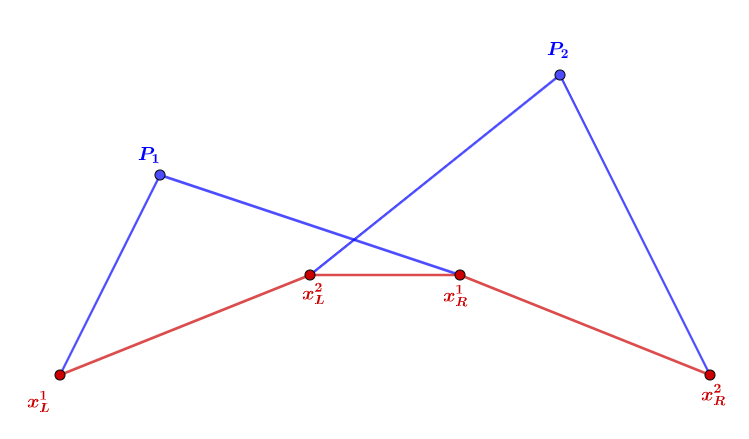
\includegraphics[width = 0.7\linewidth]{proof1.PNG}
    \caption{The mothership launches two drones sequentially}
    \label{fig:proof1}
\end{figure}

\noindent
In order to present our next result, wlog,  we restrict ourselves to the degenerate case where graphs reduce to points. The reader may note that we could reduce the general case to this one reducing the available endurance so that is possible to traverse the required percentage of these graphs. We simplify the proof considering a generic solution between two consecutive target points.


\begin{theorem}
Let $x_L^1$, $x_L^2$ (resp. $x_R^1$, $x_R^2$) be the launching (resp. rendezvous) points associated to the visit of the target points $P_1$ and $P_2$. If there exist two points $x_L$ and $x_R$ verifying 
$$
 \left\{
 \begin{array}{ccl}
  \dfrac{\|x_L-x_R\|}{v_C} & \leq    & \dfrac{\|x_L - P_1\| + \|P_1 - x_R\|}{v_D}, \\
  \dfrac{\|x_L-x_R\|}{v_C} & \leq    & \dfrac{\|x_L - P_2\| + \|P_2 - x_R\|}{v_D}, \\
  \dfrac{\|x_L-x_R\|}{v_C} & \leq   & N^d, \\
  \|x_L-x_R\| & \leq & \|x_L^1 - x_L^2\| + \|x_L^2- x_R^1\| + \|x_R^1-x_R^2\|,
 \end{array}
 \right.
$$

\noindent then the contribution of this partial route to the optimal objective value will be the same in both models.
\end{theorem}

\begin{proof}
Note that in the considered configuration, the order of visit to the points $P_1$ and $P_2$ is fixed and then, the binary variables in the model are fixed in this case. Thus, the only difference that the two models can have are the location of the launching and rendezvous points. Hence, the only constraints that are involved are those related to these points. These are the conditions in the statement: The first two are the \eqref{DCW} inequalities. The third one is the \eqref{CAP} constraint and the last one ensures that the distance traveled by the mothership in the synchronized model is smaller than or equal to the distance assumed in the non-synchronized solution described in the statement. Therefore, the conclusion follows.

\end{proof}

% Note that this result states necessary and sufficient conditions to obtain the same solution for the two models.



%(Meto restricción de capacidad? para hacer experimentos puede complicarse)

% $$
% e=(i, j) \ni x_R^t \rightarrow V_i \vee V_j \rightarrow \ldots \rightarrow V_k \rightarrow \ldots \rightarrow V_{i'} \rightarrow x_L^{t+1} \in (i',j')=e'
% $$

% The design of these paths obeys to define binary variables that decide which vertices are selected in each stage $t$: 